\documentclass[12pt]{article}

\usepackage{xcolor} % for different colour comments
\usepackage{cite}
\usepackage{hyperref}
\usepackage{graphicx}
\usepackage{float}
\usepackage[export]{adjustbox}
\usepackage{multirow}


\usepackage[%
    left=1in,%
    right=1in,%
    top=1.0in,%
    bottom=1.0in,%
    paperheight=11in,%
    paperwidth=8.5in%
]{geometry}%

%% Comments
\newif\ifcomments\commentstrue

\ifcomments
\newcommand{\authornote}[3]{\textcolor{#1}{[#3 ---#2]}}
\newcommand{\todo}[1]{\textcolor{red}{[TODO: #1]}}
\else
\newcommand{\authornote}[3]{}
\newcommand{\todo}[1]{}
\fi

\newcommand{\wss}[1]{\authornote{magenta}{SS}{#1}}
\newcommand{\hm}[1]{\authornote{blue}{HM}{#1}} %Hediyeh
\newcommand{\tz}[1]{\authornote{blue}{TZ}{#1}} %Tahereh
\newcommand{\pl}[1]{\authornote{blue}{PL}{#1}} %Peng

\begin{document}

\title{Design Document for JScrypt}
\author{Jean Lucas Ferreira, Ocean Cheung, Harit Patel}

\date{\today}

\maketitle


\newpage
  \tableofcontents

\newpage


\section{Introduction}

 This document is dedicated to documenting the the module interface specification (MIS) of JScrypt. It is intended to represent the the system’s architectural design and detailed design, and describe the levels of interaction and hierarchy of modules throughout the project. The creation of this project will facilitate developers and testers to create test cases, and find modules that can potentially violate certain design principles.

\section{Anticipated and Unlikely Changes}

The system is susceptible to many changes and have been categorized by their likelihood as anticipated changes and unlikely changes.

\subsection{Anticipated Changes}
Anticipated changes to JScrypt mainly include addition of more preferences/options that users may be able to integrate into their applications. Perhaps slight changes in encryption or decryption algorithms may be made to improve performance. \newline

AC1: Addition or changes to current options available to the users. \newline
AC2: Changes in encryption/decryption algorithms

\subsection{Unlikely Changes}
Constants used in the system will unlikely be changed. These values are common throughout various implementations of bCrypt. Changing some of these values may result with an inconsistent implementation, and will no longer be following the bCrypt standard.
Examples of these constants are:
  \begin{itemize}
    \item Salt string length
    \item P-Arrays and S-boxes values
    \item Minimum, maximum, and default rounds value
	\end{itemize}
Also, the implementation of Eksblowfish in the project will unlikely be changed in terms of data structures, function signatures, and return types. \newline

UC1: Constants: Salt String length, P-Array and S-boxes values, minimum and maximum rounds value. \newline
UC2: Implementation of EksBlowfish algorithm in terms of data structure, function signatures, and return types.

\section{Module Hierarchy}

The different design modules of JScrypt will be defined in this section. The modules listed below will be implemented into the JScrypt project.
\begin{table}[H]
  \begin{tabular}{ | p{6cm} | p{7cm}|}
    \hline
        \textbf{Level 1} & \textbf{Level 2}\\
    \hline

      Hardware-Hiding Module & N/A \\
   \hline

    Behaviour-Hiding Module & Key Expansion Module \newline Feistal Cipher Module \newline Feistal F Module  \\
   \hline

    Software Decision Module & Generate Random Salt Module \newline Hash Key Module \newline \textcolor{red}{Get Components Module} \newline Compare Key Module \\
   \hline

 \end{tabular}
\end{table}

M1: hashKey \\
M2: compareKey \\
M3: getComponents \\
M4: generateRandomSalt \\
M5: keyExpansion \\




\section{Connection between requirements and design}

	Due to some of the non-function, requirements specified in the Software Requirements Specification document, certain design decisions were made:

	\begin{enumerate}
		\item To fulfill the ease of use requirement, the library will only allow the user access to two methods. By doing so, the user is only responsible for encrypting and storing the input string.
		\item The API of the project will be provided in the git repository (through readme.md), explaining how to get started with the project, and what can be done with it. This will help satisfy the ease of use, and learning requirements of the project.
		\item The user will be provided an option to input the number of rounds the encryption algorithm should perform on the input string. This will satisfy the speed and latency requirements as the user will be able to choose the speed at which the algorithm is completed.
		\item The library will only be in use each time the library functions are called and does not make changes to the application in question. Additionally, the library will be made open-source to all developers. This will fulfill the reliability and availability requirements.


	\end{enumerate}

\section{Module Decomposition}

\subsection{Hardware Hiding Modules}

	Not Applicable for this project

\subsection{Behaviour Hiding Modules}

	\textbf{Module Name:} Hash Key
	\begin{itemize}
	  \item \textbf{Secret:} How the key is hashed
	  \item \textbf{Service:} Takes a string and hashes it
	\end{itemize}

	\textbf{Module Name:} compareKey
	\begin{itemize}
	  \item \textbf{Secret:}Compares a plaintext string with a hashed string
	  \item \textbf{Service:} Verifies if a plaintext string and hashed string are the same
	\end{itemize}

	\textbf{Module Name:} getComponents
	\begin{itemize}
	  \item \textbf{Secret:} Splices a hash key
	  \item \textbf{Service:} Certifies the hask key has an appropriate format, and separates all the componets in order to simply the compareKey
	\end{itemize}

	\textbf{Module Name:} generateRandomSalt
	\begin{itemize}
	  \item \textbf{Secret:} Generates a random salt to use when hashing strings
	  \item \textbf{Service:} Random string of 22 ASCII characters is created
	\end{itemize}

	\textbf{Module Name:} keyExpansion
	\begin{itemize}
	  \item \textbf{Secret:} Given a key (to be encrypted), represent that key as hexadecimal digits, and split it up into an array of 14 indexes, treating the key as cyclic.
	  \item \textbf{Service:}  Initiates the encryption environment based on the key.
	\end{itemize}


\section{Uses Relation}

	\begin{figure}[H]

	\centerline{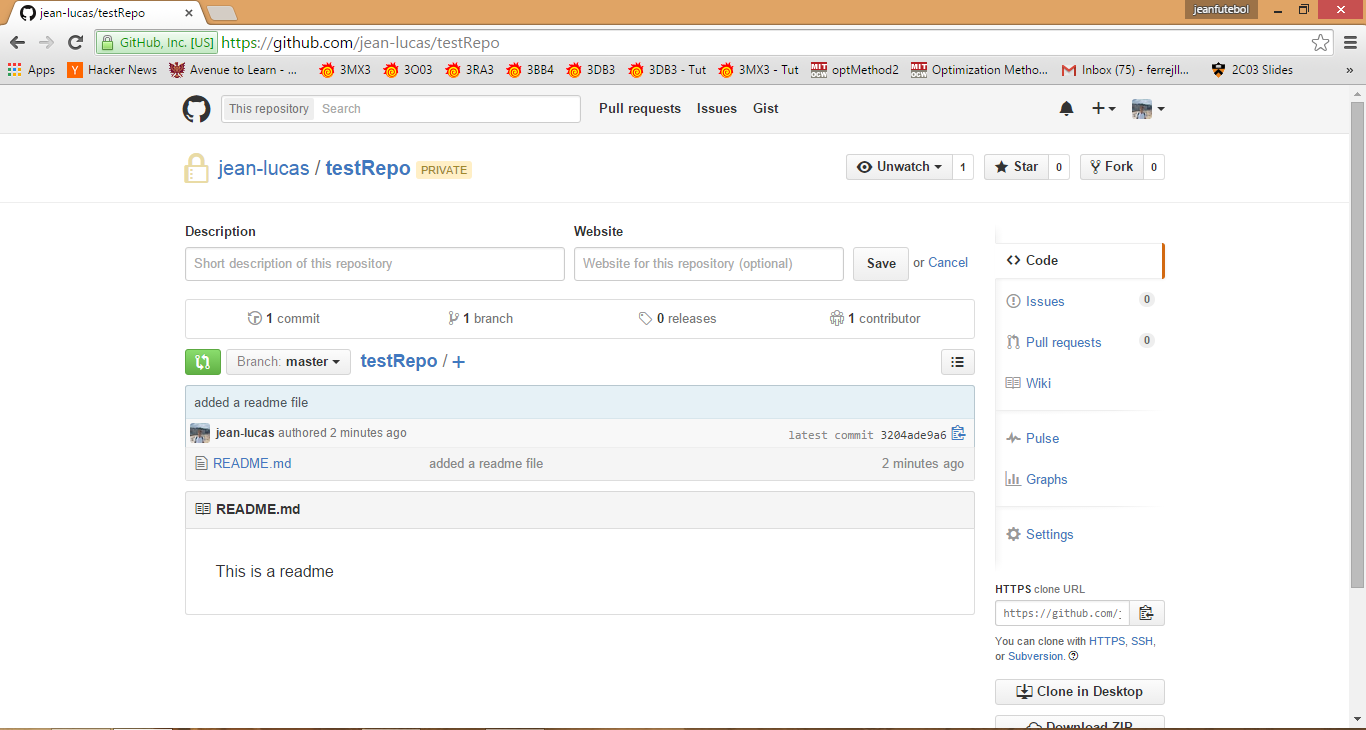
\includegraphics[width=\textwidth]{Capture3.PNG}}
	\caption{Uses Relation}
	\end{figure}


\section{Schedule}

\subsection{Pert Chart}


	\begin{figure}[H]
	\centerline{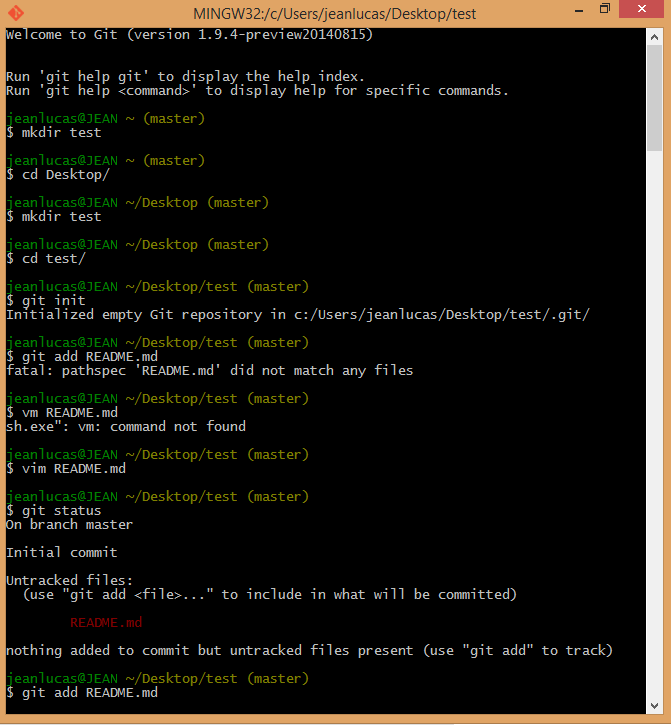
\includegraphics[width=\textwidth]{Capture.PNG}}
	\caption{Pert Chart}
	\end{figure}

\subsection{Gantt Chart}

	\begin{figure}[H]
	\centerline{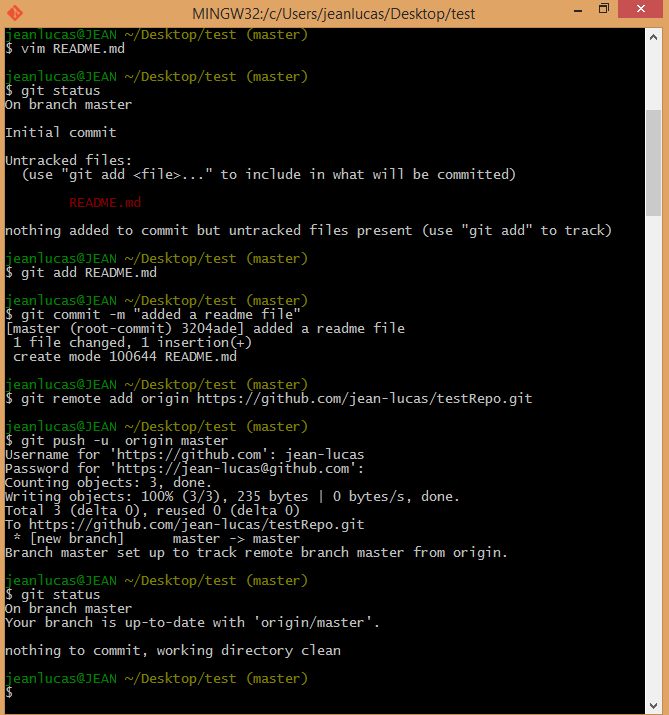
\includegraphics[width=\textwidth]{Capture2.PNG}}
	\caption{Gantt Chart}
	\end{figure}


\textcolor{red}{}
 \section{MIS for JScrypt}

 \subsection{Methods}

\textbf{compareKey(cleanKey, hashKey)}

Encrypts the string `cleanKey' and compares to see if the cleanKey is the same as hashKey after the encryption process.

\textbf{Parameters:}

\begin{table}[H]
\centering
\label{tab:table2}
      \begin{tabular}{ | p{4cm} | p{4cm} | p{9cm} | }
        \hline
            \textbf{Name} & \textbf{Type} & \textbf{Description} \\
        \hline
          cleanKey & string & plain text string that needs to be compared with hashKey  \\
        \hline
          hashKey & string & hashed string generated by the program which consists of version, number of rounds, salt, and encrypted key. \\
       \hline
      \end{tabular}
  \end{table}

Source: JScrypt.js, line 135

\textbf{generateRandomSalt(rounds)}
Generates a random padded string of length 24, which is used for hashing the key. This string includes padding which will later be removed before hashing the key.

\textbf{Parameters:}
\begin{table}[H]
\centering
\label{tab:table2}
      \begin{tabular}{ | p{4cm} | p{4cm} | p{9cm} | }
        \hline
            \textbf{Name} & \textbf{Type} & \textbf{Description} \\
        \hline
          rounds & integer & Number of times the key is hashed.  \\
       \hline
      \end{tabular}
  \end{table}
Source: JScrypt.js, line 35


\textbf{getComponents(hashKey)}

A String can go through a series of rounds to become hashed and finding the number of rounds in the components gives us the knowledge required to compare a string of plaintext to a hashed string.

\textbf{Parameters:}
\begin{table}[H]
\centering
\label{tab:table2}
      \begin{tabular}{ | p{4cm} | p{4cm} | p{9cm} | }
        \hline
            \textbf{Name} & \textbf{Type} & \textbf{Description} \\
        \hline
          hashKey & string & string generated by the encryption process with information containing the version, number of rounds, salt, and encrypted key.  \\
       \hline
      \end{tabular}
  \end{table}
Source: Jscrypt.js, line 189

\textbf{hashKey(rounds, key)}

Generates the hash string(refer to section 3.4) that will be stored in the applications database. This is the only function that a user of the project will be required to call in order to hash a string to encrypt information.

\begin{table}[H]
\centering
\label{tab:table2}
      \begin{tabular}{ | p{4cm} | p{4cm} | p{9cm} | }
        \hline
            \textbf{Name} & \textbf{Type} & \textbf{Description} \\
        \hline
          rounds & integer & integer input from 6 to 31  \\
        \hline
          key & string & string input of length 1 to 56 characters \\
       \hline
      \end{tabular}
  \end{table}

  Source: JScrypt.js, line 65


\section{MIS for eksBlowfish}

\subsection{eksblowfish}

eksBlowfish implementation

\textbf{Properties}:

\begin{table}[H]
\centering
\label{tab:table2}
      \begin{tabular}{ | p{4cm} | p{4cm} | p{9cm} | }
        \hline
            \textbf{Name} & \textbf{Type} & \textbf{Description} \\
        \hline
          keyExpansion & function & Sets up the encryption environment with the given key by setting up the P_arrays and the S_boxes with hexadecimal values of the key  \\
        \hline
          feistel_cipher & function & The heart of the encryption. Runs through a feistel network of 2^(number of rounds) times. At each iteration, the P_arrays and S_boxes are updated according to the salt and the key.  \\
        \hline
          feistal_F & function & Helper function of the Feistel_cipher
       \hline
      \end{tabular}
Source: eksBlowfish.js, line 11
  \end{table}
}

\end{document}
